% !TEX root = ./cvl.tex
\section{Experimental Results}

\marcos{Say we use PostgreSQL + PostGIS here.}
\marcos{Say that automatic parallelism is not supported natively by PostGIS, but is an interesting avenue for future work.}

Show performance, scalability and quality for algorithms and constraints, i.e. performance of "find conflicts" and "find set multicover".

\begin{figure}[htbp]
\begin{center}
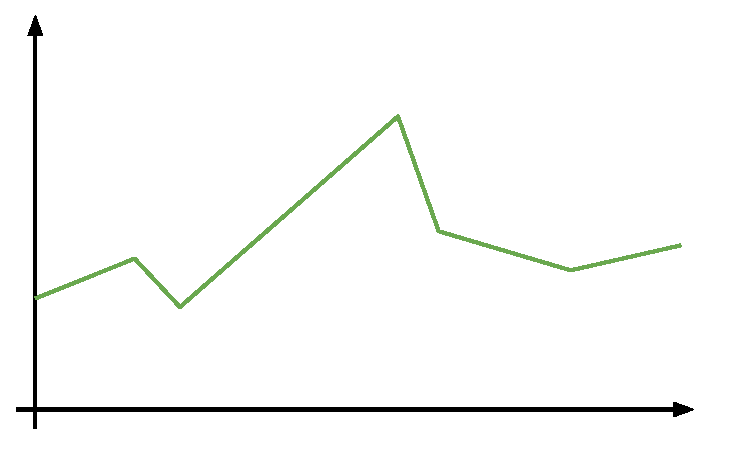
\includegraphics[scale=.5]{figs/cvl_todo.pdf}
\caption{Results for experiment.}
\label{fig:results-x}
\end{center}
\end{figure}

\begin{table}[htdp]
\caption{Datasets used in experiments}
\begin{center}
\begin{tabular}{|c|c|c|c|}
\hline
\textbf{Dataset} & \textbf{Type} & \textbf{Records} & \textbf{Points} \\
\hline
Openflights airports & Points & $7K$ & $7K$ \\
World amenities & Points & $500K$ & $500K$ \\
Synthetic aminities & Points & $30000K$ & $30000K$ \\
US Waterways & Linestrings & $500K$ & $500K$ \\
Danish Area Information & Polygons & $30K$ & $9000K$ \\
\hline
\end{tabular}
\end{center}
\label{default}
\end{table}%
